% Owners: 7.1-7.2 Cosmin, 7.3-7.6 Sergiu
\section{Optimisations}
\label{sec:opt}

Each strategy below is motivated by the analysis or the model. Every variant passes the BFS
verifier. Figure~\ref{fig:opt} summarises speed-ups on \texttt{kron20}, and
Table~\ref{tab:opt} gives medians and IQRs. Following Section~\ref{sec:method}, we call a
difference significant only if it exceeds the IQR of both configurations.

\begin{figure}[ht]
\centering
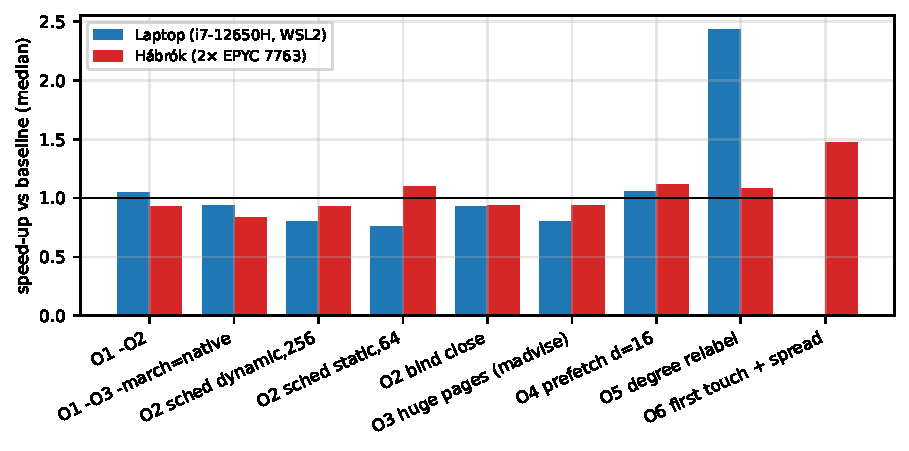
\includegraphics[width=0.9\linewidth]{figures/optimisations.pdf}
\caption{Speed-up of selected variants over the baseline (\texttt{kron20}, all threads,
ratio of medians).}
\label{fig:opt}
\end{figure}

\begin{table}[ht]
\centering\footnotesize
\caption{Median [IQR] in ms per search. Baseline: \texttt{-O3}, default schedule and threads.
Bold: significant improvement.}
\label{tab:opt}
\begin{tabular}{@{}llll@{}}
\toprule
Variant & Graph & Laptop & Hábrók \\
\midrule
Baseline & kron20 & 8.58 [4.77] & 2.85 [1.43] \\
O1 \texttt{-O0} / \texttt{-O2} / \texttt{-O3 -march=native} & kron20 & 20.3 / 8.22 / 9.16 & 7.03 / 3.07 / 3.43 \\
O2 \texttt{static,64} / \texttt{dynamic,256} (both loops) & kron20 & 11.3 / 10.7 & 2.59 [3.21] / 3.08 \\
O2 threads = 8 (laptop) / 48 (Hábrók), bound & kron20 & 8.39 [1.23] & \textbf{1.38 [0.57]} \\
O3 THP \texttt{never} / \texttt{madvise} / patch / \texttt{always} & kron20 & 9.98 / 11.75 / 10.72 / 8.24 & -- / -- / 3.05 / 2.97 \\
O3 huge-page patch & kron22 & 50.2 [43.2] vs.\ 71.1 [58.5] & 12.83 vs.\ 12.14 \\
O4 prefetch $d{=}16$ & kron20 & 8.15 [3.70] & 2.55 [1.57] \\
O5 degree relabelling & kron20 & \textbf{3.53 [1.77]} & 2.64 [3.13] \\
O5 degree relabelling & kron22 & \textbf{25.1 [12.8]} vs.\ 71.1 & \textbf{6.67 [1.35]} vs.\ 12.14 [1.66] \\
O5 degree relabelling & kron24 & -- & 33.7 [17.3] vs.\ 38.2 [5.7] \\
O6 base vs.\ first touch, spread binding & kron20 & -- & 4.00 [1.17] vs.\ \textbf{1.94 [1.18]} \\
O6 base vs.\ first touch, spread binding & kron22 & -- & 12.33 [1.21] vs.\ \textbf{10.96 [1.35]} \\
O7 $\alpha{=}15,\beta{=}9$ / $\alpha{=}5,\beta{=}9$ & kron20 & 8.17 / 37.8 & 2.42 [1.34] / 2.76 \\
\bottomrule
\end{tabular}
\end{table}

\subsection{O1: Compiler optimisation and vectorisation}
\emph{Rationale.} This is the cheapest lever, and it is in our work plan. \emph{Result.}
\texttt{-O0} is 2.4$\times$ slower than \texttt{-O3} on both machines; \texttt{-O1} recovers
most of it; \texttt{-O2} and \texttt{-O3} are indistinguishable within the IQR.
\texttt{-march=native} is not faster (\SI{9.16}{ms} vs.\ \SI{8.01}{ms} on the laptop,
\SI{3.43}{ms} vs.\ \SI{2.75}{ms} on Hábrók, both within the IQR). The GCC vectorisation
report explains why: no hot loop is vectorised. The \texttt{BUStep} inner loop is rejected
because of \emph{control flow in loop} (the early \texttt{break}), its outer loop because of
\emph{multiple nested loops}, and \texttt{TDStep} because the atomic compare-and-swap
\emph{clobbers memory}. Vectorising BFS would need a different algorithm formulation. For
the same reason we did not apply the classic loop transformations (unrolling, unroll-and-jam,
interchange): BFS's loops have data-dependent trip counts and early exits, and
\texttt{-O3} already unrolls where possible. The model also shows the bottleneck is in the
memory system, so the instruction count matters little once \texttt{-O1} has removed the
gross overhead.

\subsection{O2: OpenMP scheduling, binding and thread count}
\emph{Rationale.} Half of the samples are spent in the OpenMP runtime
(Table~\ref{tab:hotspots}), and on Hábrók the model leaves a factor 2.5--6.5 unexplained
(Section~\ref{sec:model}). \emph{Change.} \texttt{schedule(runtime)} for both step loops,
swept over chunk sizes that are multiples of 64 (Section~\ref{sec:method}); thread binding;
thread count. \emph{Result.} No schedule beats the upstream combination (static top-down,
\texttt{dynamic,1024} bottom-up). Applying one schedule to both loops is worse on the laptop,
and Hábrók's best (\texttt{static,64}, \SI{2.59}{ms}) is within the IQR. Binding alone is not
significant. Choosing the thread count is significant: on Hábrók, 48 threads bound to
consecutive cores (\SI{1.38}{ms}) are \textbf{2.1$\times$ faster} than the default 128
unbound threads. They stay on one socket, avoid cross-socket coherence traffic, and pay for
smaller barriers. On the laptop the optimum is 8 of 10 vCPUs, which is not significant.

\subsection{O3: Huge pages}
\emph{Rationale.} The latency curve (Figure~\ref{fig:latency}) rises beyond the TLB reach,
and \texttt{BUStep} and \texttt{TDStep} access a \SI{136}{MB} CSR at random. \emph{Change.}
\texttt{madvise(MADV\_HUGEPAGE)} on the CSR arrays and \texttt{pvector}s before first touch;
we confirmed with \texttt{/proc/self/smaps\_rollup} that \SI{127}{MB} of the process then uses
\SI{2}{MB} pages, against 0 without the patch. \emph{Result.} On \texttt{kron20} all four
laptop configurations lie within each other's IQR. On \texttt{kron22} the patch reduces the
laptop median by \SI{29}{\percent}, but with IQRs above \SI{40}{ms} this is not significant.
Hábrók already runs with THP \texttt{always}, so the baseline uses huge pages and the patch
changes nothing: \num{4200} vs.\ \num{4900} dTLB misses per search, both negligible against
about 2 million random accesses. On the laptop, where TLB misses inflate DRAM latency
(Figure~\ref{fig:latency}), the expected benefit is masked by WSL2's variance.

\subsection{O4: Software prefetching in top-down}
\emph{Rationale.} \texttt{TDStep}'s random \texttt{parent[v]} accesses are latency-bound, and
prefetching $d$ neighbours ahead should increase memory-level parallelism. \emph{Result.}
No distance is significant on either machine (best: $d{=}16$ on Hábrók, $-$\SI{11}{\percent},
within the IQR). The analysis predicts this. Top-down accounts for only \SI{3}{\percent} of the
samples and \SI{11}{\percent} of the modelled traffic, so even perfect prefetching could save
a few per cent (Amdahl's law). The bottom-up step, where the time goes, already issues
independent loads for consecutive vertices, which the out-of-order core overlaps.

\subsection{O5: Degree-ordered relabelling}
\emph{Rationale.} The model says the dominant traffic is one neighbour-list line per vertex
checked in bottom-up, plus random accesses to \texttt{parent}. Renumbering vertices by
decreasing degree (\texttt{-DRELABEL}, using \gapbs' \texttt{RelabelByDegree}) gives the hubs
small, adjacent IDs, which improves locality. Because neighbour lists are sorted, hubs, which
are most likely to be in the frontier, also come first in every list. \emph{Result.} This
is the most effective optimisation: \textbf{2.4$\times$} on the laptop (\texttt{kron20}),
\textbf{2.8$\times$} on the laptop and \textbf{1.8$\times$} on Hábrók for \texttt{kron22}. Our
edge counters show why it works: relabelling reduces the edges examined per search by
\SI{35}{\percent} (\texttt{kron20}) and \SI{48}{\percent} (\texttt{kron22}), because
bottom-up finds a frontier parent sooner. So it reduces both $Q$ and the work. On
\texttt{kron24} the gain is not significant (1.13$\times$, IQR \SI{17}{ms}).
\emph{Caveats.} The one-off relabelling (\SI{0.46}{s} for \texttt{kron20}) is excluded from
the search time and pays off after about 90 laptop searches. Relabelled graphs have different
vertex IDs, so the pseudo-random sources differ from the baseline's.

\begin{figure}[ht]
\centering
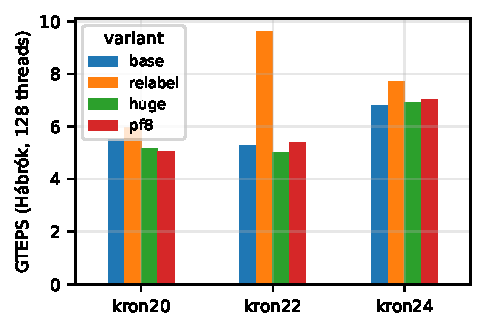
\includegraphics[width=0.48\linewidth]{figures/big_graphs.pdf}
\caption{GTEPS on Hábrók for growing graphs: relabelling helps most on \texttt{kron22}; huge
pages and prefetching do not matter on this node.}
\label{fig:big}
\end{figure}

\subsection{O6: NUMA-aware first touch}
\emph{Rationale.} Loading the graph with a single \texttt{read()} touches every page from one
thread, so on Hábrók the whole \SI{125}{MB} edge array lands on one socket. The second
socket's threads then read everything remotely, and only one socket's memory controllers are
used. \texttt{numactl} is not available, so \emph{change}: \texttt{-DPAR\_FIRST\_TOUCH}
zeroes the array in parallel before reading. \emph{Result.} Placement matters as soon as
threads are spread over both sockets. With \texttt{OMP\_PROC\_BIND=spread}, the baseline
slows to \SI{4.00}{ms} [IQR 1.17] on \texttt{kron20}, because half of the threads read
everything remotely. With parallel first touch it takes \textbf{\SI{1.94}{ms} [1.18], a
2.1$\times$ improvement}, and 1.5$\times$ faster than the default configuration. On
\texttt{kron22} first touch gains \SI{11}{\percent} with spread binding (\SI{12.33}{} $\to$
\SI{10.96}{ms}, significant). Unbound, the gains are smaller and within the IQR, because the
OS places threads unpredictably. On \texttt{kron24} the difference is not significant; we have
not yet determined why the effect disappears for the largest graph.

\subsection{O7: Direction-switch thresholds}
\emph{Rationale.} $\alpha$ and $\beta$ decide how much work runs in the two very different
steps. \emph{Result.} A $3\times3$ sweep shows the defaults are near-optimal. $\alpha{=}5$
keeps the search top-down for too long and is 4.4$\times$ slower on the laptop. The best
settings ($\alpha{=}15,\beta{=}36$ on the laptop, $\alpha{=}15,\beta{=}9$ on Hábrók) are
within the IQR of the defaults.
